\section{Les bases de données NoSQL:}
Depuis les années 70, la base de données relationnelle était l'incontournable référence pour gérer les données d'un système d'information. Toutefois, face aux 3V (Volume, Velocity, Variety), le relationnel peut difficilement lutter contre cette vague de données. Le NoSQL s'est naturellement imposé dans ce contexte en proposant une nouvelle façon de gérer les données, sans reposer sur le paradigme relationnel, d'où le "Not Only SQL". Cette approche propose de relâcher certaines contraintes lourdes du relationnel pour favoriser la distribution (structure des données, langage d'interrogation ou la cohérence).

\subsection{Définition : }
En informatique et en bases de données, NoSQL désigne une famille de systèmes de gestion de base de données (SGBD) qui s'écarte du paradigme classique des bases relationnelles. L'explicitation la plus populaire de l'acronyme est Not only SQL (« pas seulement SQL » en anglais) et c'est en effet ce que ce modèle de base
de données veut être : non pas une contrepartie, mais bien un enrichissement et complément utile des bases de données SQL relationnelles traditionnelles. Ce faisant, les bases de données NoSQL dépassent les limites des systèmes relationnels et exploitent un modèle de base de données alternatif. Cela ne veut toutefois pas dire qu'aucun système SQL n'est utilisé. Il existe de nombreuses variantes combinées au sein desquelles les deux solutions peuvent être utilisées et qui restent toutefois englobées sous l'étiquette NoSQL.

La définition exacte de la famille des SGBD NoSQL reste sujette à débat. Le terme se rattache autant à des caractéristiques techniques qu'à une génération historique de SGBD qui a émergé autour des années 2010. D'après Pramod J. Sadalage et Martin Fowler, la raison principale de l'émergence et de l'adoption des SGBD NoSQL serait le développement des centres de données et la nécessité de posséder un paradigme de bases de données adapté à ce modèle d'infrastructure matérielle.
\begin{itemize}[label=\textbullet]
\item \textbf{Distinction des autres termes :}
\begin{itemize}[label=\textbullet]
\item \textbf{Non SQL :} Le terme « bases de données non SQL » est trompeur, pour ne pas dire faux. Il prédit que ces bases de données sont sans aucune utilisation de SQL et ce n'est pas toujours le cas dans NoSQL. Le terme bases de données non SQL existe, mais il est plutôt utilisé comme un terme vague que comme une expression professionnelle. Cela signifie que les données sont traitées par un autre langage que SQL, par ex. XQuery pour les bases de données XML.
\item \textbf{Distributed storage :} Liés à NoSQL, il existe des termes tels que « stockage distribué » ou « stockage structuré distribué ». Il est assez difficile de distinguer ces termes de NoSQL, car ils décrivent exactement une caractéristique de NoSQL. Le stockage distribué est un terme générique pour un système qui prétend être un stockage unique mais qui est en réalité une collection de nombreuses unités informatiques stockant des parties des fichiers. Certaines bases de données NoSQL prétendent être un système de stockage distribué, par exemple BigTable de Google.
\end{itemize}
\end{itemize}
\newpage
\subsection{Théorème de CAP: }
Le théorème de CAP est l’acronyme de « Coherence », « Availability » et « Partition tolerance », aussi connu sous le nom de théorème de Brewer. Ce théorème, formulé par Eric Brewer en 2000 et démontré par Seth Gilbert et Nancy Lych en 20025, énonce une conjecture qui définit qu’il est impossible, sur un système informatique de calcul distribué, de garantir en même temps les trois contraintes suivantes :

\begin{itemize}[label=\textbullet]
\item \textbf{« Coherence » (Cohérence) :} Tous les clients du système voient les mêmes données au même instant.
\item \textbf{« Availibility » (Haute disponibilité) :} Un système est dit disponible si toute requête reçue par un noeud retourne un résultat. Bien évidemment le noeud en question ne doit en aucun cas être victime de défaillance.
\item \textbf{« Partition tolerance » (Tolérance à la partition) :} Un système est dit tolérant à la partition s’il continue à répondre aux requêtes de manière correcte même en cas de panne autre qu’une panne totale du système.
\end{itemize}

\begin{figure}[h]
	\centering
    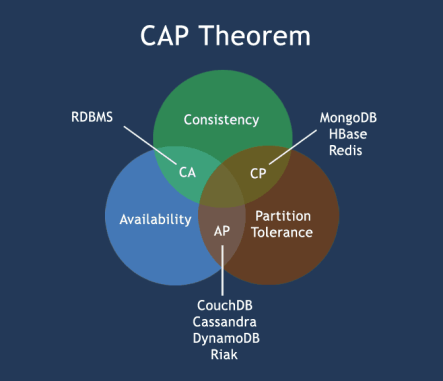
\includegraphics[scale=0.5]{img/4.1}
    \caption{Théorème de CAP}
\end{figure}

Seules deux des trois contraintes peuvent être respectées en même temps. Un des premiers buts des systèmes NoSQL est de renforcer la « scalabilité » horizontale, il faut pour cela que le principe de tolérance au partitionnement soit respecté, ce qui exige l’abandon soit de la cohérence, soit de la haute disponibilité.

\subsubsection{Haute disponibilité et tolérance à la partition: (AP)}
Les bases ne sont pas forcément cohérentes dans le temps mais la multiplicité des bases sur le réseau permet de garantir une réponse quoi qu'il arrive.

En effet, cela voudrait dire que les utilisateurs n’ont pas forcément tous la même vue à un moment donné. Dans certains cas cela peut poser des problèmes, mais bien souvent ce n’est pas une nécessité. Prenons l’exemple de deux utilisateurs qui sont amis sur Facebook, Marcel et Pierre. Si Marcel partage une photo sur son « mur » et que Pierre au même instant ne la voit pas dans son « fil d’actualité » elle apparaîtra dans les prochaines secondes. Dans ce cas précis, est-ce un problème pour Pierre d’attendre environ une minute pour voir la photo que vient de publier son ami Marcel ?

\subsubsection{Cohérence et tolérance à la partition: (CP)}
Un tel système de base de données stocke les données dans les nœuds distribués, mais assure également la cohérence de ces données, mais le support n'est pas assez bon pour la disponibilité.

La plupart du temps, les systèmes NoSQL qui garantissent une forte cohérence des données sont architecturés en maître/esclave. Cela veut dire que toutes les écritures doivent être faites sur le serveur maître, et en cas de panne de ce dernier, les opérations d’écriture, de modification et de suppression ne deviennent plus disponibles. Seule la lecture des données sur les serveurs esclaves est possible.

\subsubsection{Cohérence et Haute disponibilité (CA):}
Tous les clients du système voient les mêmes données au même instant. Notamment les deux propriétés respectées par les bases de données relationnelles. 


\subsection{Les propriétés de BASE : }
Dans la première partie consacrée aux bases de données relationnelles nous avons vu les propriétés ACID auxquelles doivent répondre les SGBD de type relationnel. Les SGBD NoSQL qui, selon le théorème CAP, privilégient la disponibilité ainsi que la tolérance à la partition plutôt que la cohérence, répondent aux propriétés de BASE.

Le principe de BASE est le fruit d’une réflexion menée par Eric Brewer (Théorème de CAP). Les caractéristiques de BASE sont fondées sur les limites que montrent les SGBD relationnelles. Voici sa description :
\begin{itemize}[label=\textbullet]
\item \textbf{Basically Available :} quelle que soit la charge de la base de données (données/requêtes), le système garantie un taux de disponibilité de la donnée.
\item \textbf{Soft-state :} La base peut changer lors des mises à jour ou lors d'ajout/suppression de serveurs. La base NoSQL n'a pas à être cohérente à tout instant.
\item \textbf{Eventually consistent :} À terme, la base atteindra un état cohérent.
\end{itemize}

\begin{figure}[h]
	\centering
    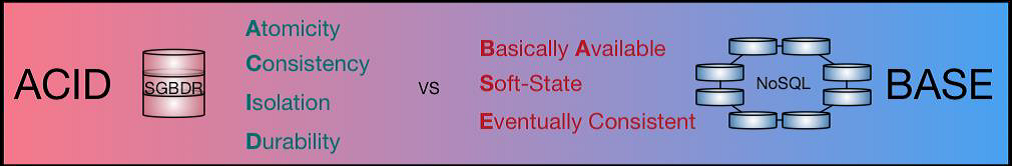
\includegraphics[scale=0.5]{img/4.2}
    \caption{ACID vs BASE}
\end{figure}

Ainsi, une base NoSQL relâche certaines contraintes, telles que la synchronisation des réplicas, pour favoriser l'efficacité. Le parallèle ACID / BASE repris du domaine de la chimie permet d'appuyer là où ça fait mal : la concurrence. L'enfer des transactions gérées par les bases de données relationnelles est transformé en paradis pour le temps de réponse en relâchant cette contrainte impossible à maintenir.
\newpage
\subsection{Les types de bases de données NoSql :}
Dans la mouvance NoSQL, il existe une diversité d’approches classées en quatre catégories. Ces différents systèmes NoSQL utilisent des technologies forts distinctes. Les différents modèles de structure sont décrits comme suit :

\subsubsection{Les bases de données orientées clé-valeur:}
Souvent assimilé à une « hashmap » distribuée, le système de base de données de type clé/valeur est probablement le plus connu et le plus basique que comporte la mouvance NoSQL. Son principe est extrêmement simple : chaque objet (valeur) est identifié par une clé unique. Celle-ci représente la seule manière de solliciter l’objet.

La communication avec la base de données se résume aux opérations basiques que sont PUT, GET, UPDATE et DELETE. La plupart des bases de données de type clé/valeur disposent d’une interface HTTP REST qui permet de procéder très facilement à des requêtes depuis n’importe quel langage de développement. Ces systèmes affichent des performances exceptionnellement élevées en lecture et en écriture, ainsi qu’une « scalabilité » horizontale étendue, cela vient du fait que ces types de bases sont réduits à un simple accès disque.

Du fait que les opérations possibles soient basiques (simple CRUD), le besoin en « scalabilité » verticale est fortement réduit. Ces systèmes sont souvent utilisés comme dépôts de données si toutefois les besoins en termes de requêtes restent de niveau simple et que l’intégrité relationnelle des données est non significative.

\begin{figure}[h]
	\centering
    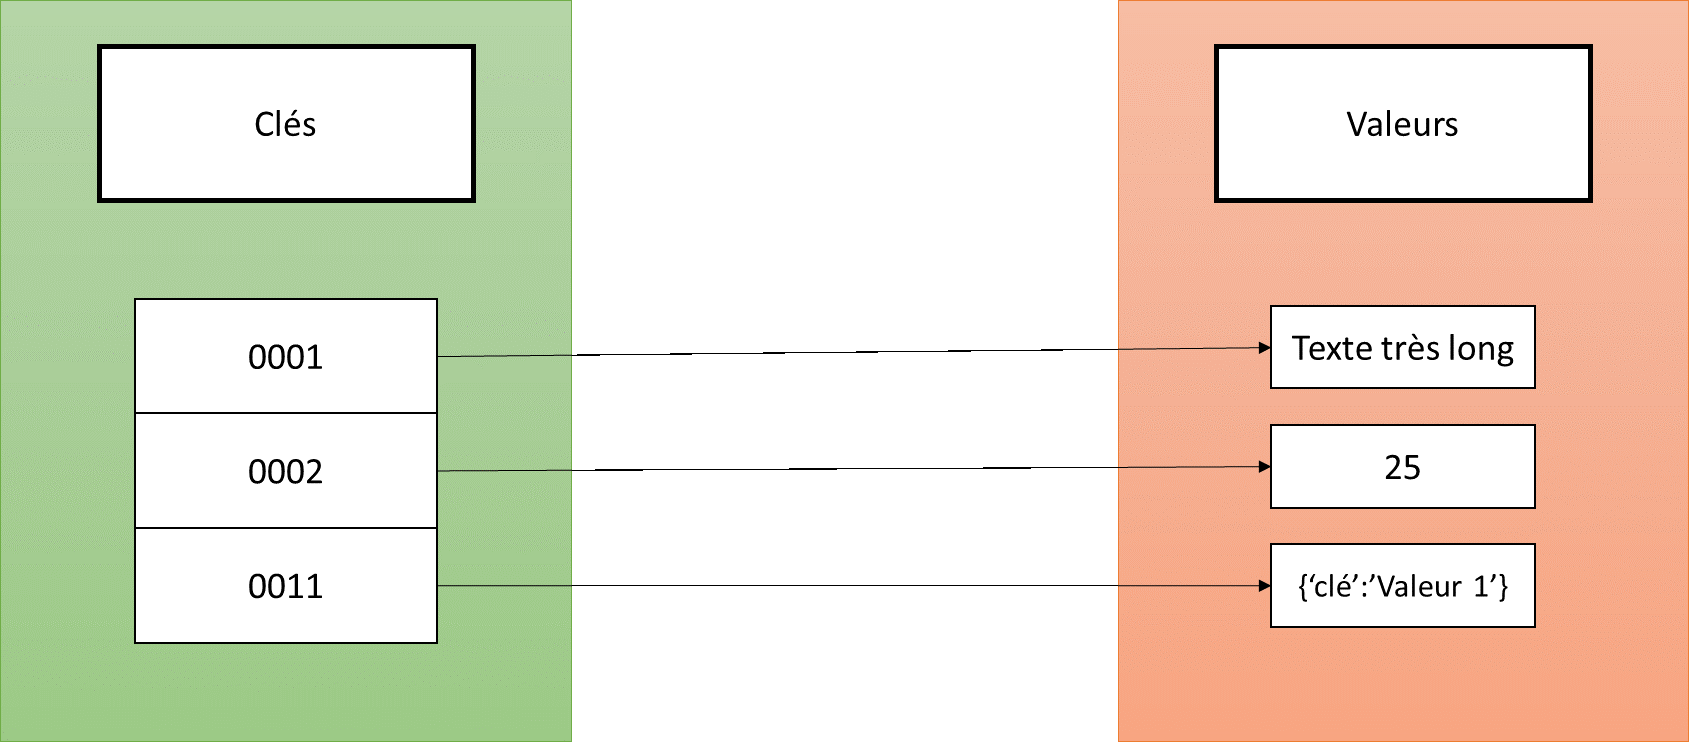
\includegraphics[scale=0.5]{img/4.3}
    \caption{base de donnée orientée clé-valeur}
\end{figure}

\textit{\textbf{Exemple d'applications :} Détection de fraude en temps réel, IoT, e-commerce, gestion de cache, transactions rapides.}

\subsubsection{Les bases de données orientées colonnes}
La représentation orientée colonnes est celle qui se rapproche le plus des tables dans une base de données relationnelles. Elles permettent d'être beaucoup plus évolutive et flexible puisqu'on peut disposer de colonnes différentes pour chaque ligne. Elles peuvent évoluer dynamiquement en nombre et en nom et contrairement à une table relationnelle (pas de champ « NULL »).

\begin{figure}[h]
	\centering
    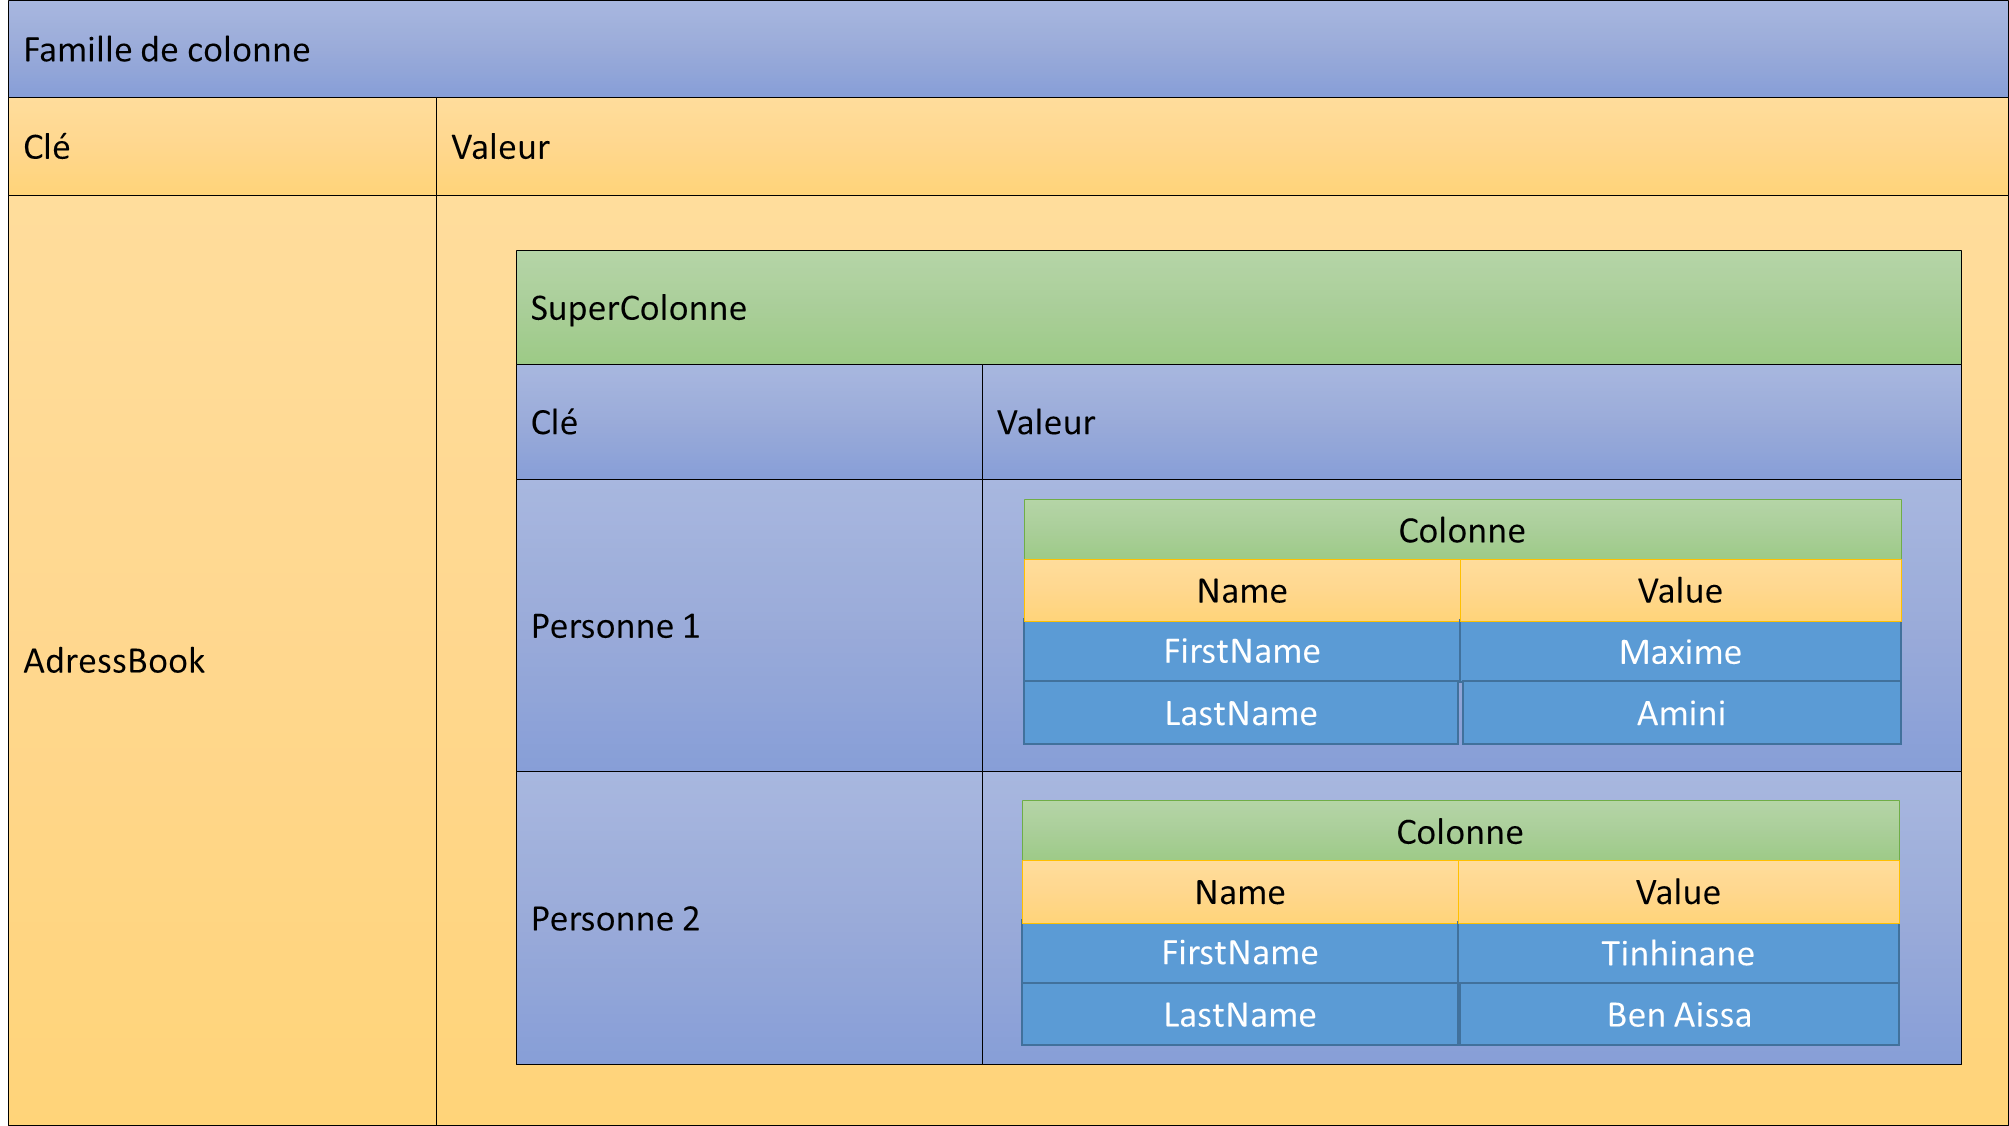
\includegraphics[scale=0.26]{img/4.4}
    \caption{base de donnée orientée colonne}
\end{figure}
\bigskip \bigskip \bigskip  \bigskip  \bigskip 
\begin{itemize}[label=\textbullet]
\item \textbf{Column :} c’est l’entité de base qui représente un champ de données. Toutes les colonnes sont définies par un couple clé/valeur
\item \textbf{Super column :} c’est une colonne qui contient d’autres colonnes
\item \textbf{Column family :} elle est considérée comme un conteneur de plusieurs colonnes ou super-colonnes
\end{itemize}

\textit{\textbf{Exemple d'applications :} Comptage (vote en ligne, compteur, etc), journalisation, recherche de produits dans une catégorie, reportage à large échelle.}

\subsubsection{Les bases de données orientées documents}
Les systèmes de type documentaire sont composés de collections de documents. La représentation en document est une sorte d’extension du concept clé/valeur. La valeur est représentée sous forme de document, ces documents ont une structure arborescente : il contient une liste de champs, un champ est associé à une valeur qui peut, elle même être une liste. Ces documents sont principalement de type JSON ou XML.

Ces bases sont dites \textbf{« Schemaless »} ce qui signifie sans schéma défini. Cela veut tout simplement dire qu’il n’est pas nécessaire de définir au préalable les champs dans le document : on peut très bien en rajouter en cours de développement. Les documents peuvent être très différents les uns des autres au sein de la base. Le fait que les documents soient structurés permet d’effectuer des requêtes sur le contenu des objets.

\begin{figure}[h]
	\centering
    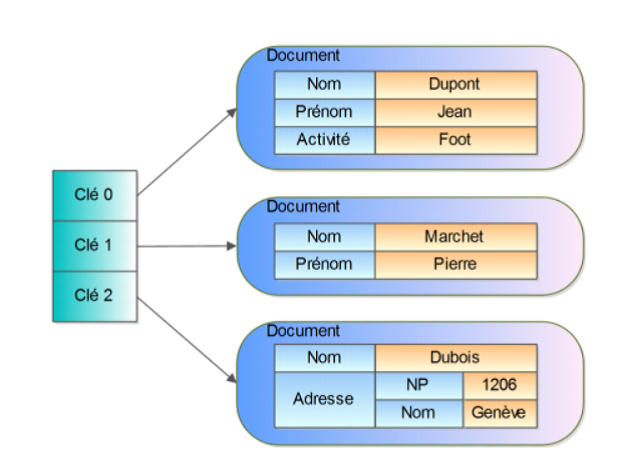
\includegraphics[scale=0.5]{img/4.5}
    \caption{base de donnée orientée document}
\end{figure}

\textit{\textbf{Exemple d'applications :} Gestion de contenu (bibliothèques numériques, collections de produits, dépôts de logiciels, collections multimédia, etc.), framework stockant des objets, collection d'événements complexes, gestion des historiques d'utilisateurs sur réseaux sociaux.}

\subsubsection{Les bases de données orientées graphes}
Une base de données graphe établit des relations entre les données à l'aide de nœuds et d'arêtes. Le réseau de relation des données est organisé par les points nodaux et leurs connexions les uns avec les autres. Dans le cas de volumes de données aux informations fortement interconnectées, les bases de données graphiques NoSQL présentent une performance considérablement supérieure à celle des bases de données SQL relationnelles. 

Elles sont principalement utilisées dans le domaine des réseaux sociaux, pour représenter, par exemple, les relations entre les abonnés sur Twitter ou Instagram.

\begin{figure}[h]
	\centering
    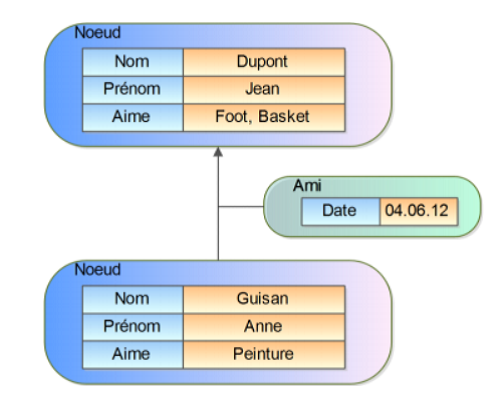
\includegraphics[scale=0.5]{img/4.6}
    \caption{base de donnée orientée graphe}
\end{figure}

\textit{\textbf{Exemple d'applications :} Réseaux sociaux (recommandation, plus court chemin, cluster...), réseaux SIG 12 (routes, réseau électrique, fret...), web social (Linked Data).}

\subsubsection{Autres base de données}
Il existe plusieurs autres bases de données suivant une approche non relationnelle, mais elles ne sont pas considérées comme des bases de données NoSQL de base, mais plutôt comme des bases de données NoSQL logicielles :

\paragraph{Bases de données d'objets :} Les bases de données d'objets utilisent l'idée d'objets dans les langages de programmation et la transforment en systèmes de bases de données.

\textit{\textbf{Exemple :} db4o est un système de gestion de base de données orientée objet Open Source pour des applications Java et .Net 13.}

\paragraph{Bases de données XML :} Les bases de données XML sont vraiment des bases de données non SQL. Le langage de requête est XQuery, XPath ou XUpdate et non plus SQL. Ces bases de données permettent de stocker des données au format XML. Par conséquent, la structure de la base de données est hiérarchique. XML est largement utilisé dans les applications Internet, donc une transformation de (anciennement) SQL en XML n'est plus nécessaire.

\textit{\textbf{Exemple :} eXist est une base de données XML basée sur Java open source prenant en charge XQuery et XPath et possède comme CouchDB une interface HTTP RESTful.}



\newpage
\subsection{Les avantages NoSQL : }
Les bases de données NoSQL ont été créées en réponse aux limitations de la technologie de base de données relationnelle. Comparées aux bases de données relationnelles, les bases de données NoSQL sont plus évolutives et offrent des performances supérieures, et leur modèle de données corrige plusieurs faiblesses du modèle relationnel. Les avantages de NoSQL sont notamment :

\begin{itemize}
\item \textbf{Gros volume de données « Big data » :} le NoSql est capable de gérer un volume important de données structurées, semi-structurées et non structurées, en effet il est devenu quasi impossible, pour un unique serveur de base de données relationnelle, de répondre aux exigences des entreprises en terme de performance. Aujourd’hui, ces gros volumes de données ne sont plus un problème pour les SGBD de type NoSQL, même le plus grand des SGBD relationnel ne peut rivaliser avec une base NoSQL.

\item \textbf{Rapidité :} NoSQL n'est pas relationnelle. Pas de schéma de bases avec les contraintes sur les champs. Cela apporte de la flexibilité dans la gestion des données et la rapidité.

\item \textbf{Modèle de données flexible :} Changer le modèle de données est une vraie prise de tête dans une base de données relationnelle en production. Les systèmes NoSQL sont plus souples en termes de modèles de données, comme dans les catégories clé/valeur et documentaire. Même les modèles un peu plus stricts comme dans la catégorie orientée colonne permettent d’ajouter une colonne sans trop de problème.

\item \textbf{Solution économique :} Les bases de données NoSQL ont tendance à utiliser des serveurs bas de gamme dont le coût est moindre afin d’équiper les « clusters », tandis que les SGBD relationnels, eux, tendent à utiliser des serveurs ultra puissants dont le coût est extrêmement élevé. De ce fait, les systèmes NoSQL permettent de revoir à la baisse les coûts d’une entreprise en termes de gigabytes ou de transactions par seconde. Cela permet de stocker ainsi que de manipuler plus d’informations à un coût nettement inférieur.
\end{itemize}
\input{part1/chapitre4/3.6_inconvénients}
\newpage
\subsection{Examples BDD NoSql : }
A l’heure actuelle, il y a plus de 122 solutions NoSQL tous types confondus (Clé/valeur, Document, Colonne et Graphe) sur le marché. La plupart d’entre elles sont soit sous licence Open Source ou soit proposées en SaaS. Les principaux contributeurs (Facebook, Google, Linkedin,…) de ces produits ont développé leurs outils à l’interne avec pour unique but de répondre à leurs propres besoins et non pas dans le but de les commercialiser. Lorsqu’ils se sont trouvés dans un état d’avancement très important (mise en production à l’interne), ces fameux SGBD ont été libérés et mis à disposition du grand public. Il ne faut pas oublier que la fondation Apache joue un grand rôle dans ces divers projets.

On citera quelques-unes classés selon leurs catégories (Pour avoir un plus large aperçu, le site nosql-database.org répertorie tous les produits de type NoSQL):

\subsubsection{BDDs orientés clé-valeur :}

\begin{itemize}[label=\textbullet]
\item \textbf{REDIS}.
\item ORACLE NOSQL.
\item \textbf{VOLDEMORT}.
\item RIAK.
\item INFINISPAN.
\item HAZELCAST.
\end{itemize}

\paragraph{1. Redis:}
Est un projet Open Source de type clé/valeur sous licence BSD. Il dispose de plus de fonctionnalités que la majeure partie des autres solutions du même type. Redis prend en charge certains langages C++, PHP, Ruby,
Python, Perl, Scala, etc. Redis est fait en langage C.

En revanche, un des seuls points négatifs à noter est que Redis ne fournit pas de réel mécanisme de partitionnement, mais uniquement une réplication de type maître/esclave. Malgré cela Redis reste très performant. Il faut aussi ajouter que le projet est sponsorisé par la société VM Ware, ce qui rend la solution crédible et pérenne.

Redis offre les caractéristiques suivantes :
\begin{itemize}[label=\ding{51}]
\item Basculement automatique (sans intervention humaine).
\item Conserve sa base de données entièrement en mémoire.
\item Les transactions sont un moyen d'envoyer en une seule opération un ensemble d'actions.
\item Répliquer les données à un nombre quelconque d'esclaves.
\item Possibilité de contrôler la durée de vie d'une donnée dans la base.
\item Prise en charge de la publication / abonnement.
\end{itemize}
\begin{figure}[h]
	\centering
    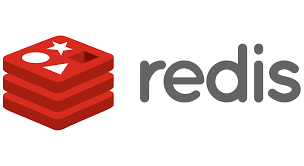
\includegraphics[scale=0.4]{img/part1/4.7}
    \caption{Logo Redis}
\end{figure}
\paragraph{2. Voldemort:}
Est un projet Open Source de type clé/valeur sous licence Apache 2.0. Il a été nommé d’après un personnage du célèbre film « Harry Potter » et offre les caractéristiques suivantes:

\begin{itemize}[label=\ding{51}]
\item Les données sont automatiquement répliquées sur de nombreux serveurs
\item Les données sont automatiquement partitionnées afin que chacun des serveurs obtienne un sous-ensemble d’un ensemble de données
\item L’échec d’un serveur est géré de manière transparente
\item Les données sont « versionnées »
\item Chaque noeud est indépendant des autres. De plus, chaque noeud du système atteint de hauts niveaux de performance de l’ordre des 20Ko d’opérations par seconde.
\end{itemize}

Le projet Voldemort développé par les ingénieurs de LinkedIn a été mis en production à l’interne en 2009. Chez LinkedIn, Voldemort est utilisé pour certaines opérations de stockage de gros volumes de données, ce qui exige des performances accrues auxquelles les solutions de stockage simple ne peuvent répondre.

\begin{figure}[h]
	\centering
    
\includegraphics[scale=0.5]{img/part1/4.8}
    \caption{Logo Voldemort}
\end{figure}

\subsubsection{BDDs orientés colonnes :}

\begin{itemize}[label=\textbullet]
\item \textbf{HBASE.}
\item \textbf{CASSANDRA}
\item ACCUMULO.
\item HYPERTABLE.
\end{itemize}

\paragraph{1. HBASE:}
HBase est une base de données distribuée et non relationnelle qui est conçue pour la base de données BigTable par Google. L'un des principaux objectifs de HBase est d'héberger des milliards (de lignes x millions de colonnes). On peut ajouter des serveurs à tout moment pour augmenter la capacité. Et de multiples nœuds maîtres assureront une haute disponibilité des données. Il est composé en Java 8. Il est autorisé sous Apache et est accompagné d'une API Java simple d'utilisation pour l'accès des clients.

Caractéristiques :
\begin{itemize}[label=\ding{51}]
\item Prise en charge de l'échec automatique.
\item Linéairement évolutif.
\item Permet la réplication des données.
\item S'intègre à Hadoop, à la fois comme source et comme destination.
\end{itemize}

\begin{figure}[h]
	\centering
    
\includegraphics[scale=0.4]{img/part1/4.9}
    \caption{Logo HBASE}
\end{figure}

\paragraph{2. CASSANDRA:}
Cassandra est une solution de type orienté colonnes. Mise en Open Source par Facebook en 2008, c’est la fondation Apache qui a repris le flambeau et l’a mise sous licence Apache 2.0. Les caractéristiques de cette solution sont les suivantes:

\begin{itemize}[label=\ding{51}]
\item flexibilité du schéma : chaque « table » est libre de suivre sa propre structure.
\item représentation spatiale de la donnée (cela permet de traiter un grand nombre de lignes)
\item « scalabilité » horizontale : s’il y a besoin de plus de puissance, on rajoute un serveur au cluster.
\item plusieurs niveaux de stratégie de cohérence des données en écriture.
\item réplication multi data-center.
\end{itemize}

Cassandra est utilisée par de nombreux acteurs de premier plan comme Facebook, Twitter et Cisco. Ceci garantit une certaine pérennité du produit. De plus une vaste communauté d’utilisateurs fait partager ses connaissances du produit et le font évoluer.

\begin{figure}[h]
	\centering
    
\includegraphics[scale=0.1]{img/part1/4.10}
    \caption{Logo CASSANDRA}
\end{figure}

\subsubsection{BDDs orientés documents :}

\begin{itemize}[label=\textbullet]
\item \textbf{MONGODB.}
\item  \textbf{COUCHDB.}
\item  RAVENDB.
\item  JERRASTORE.
\end{itemize}

\paragraph{1. MONGODB:}
MangoDB est un système de la catégorie orientée documents, le plus populaire de sa catégorie. Il est écrit en C++ et Open Source sous licence AGPL v3.0. Cette solution a été développée par la société 10gen. Voici les caractéristiques du produit:

\begin{itemize}[label=\ding{51}]
\item flexibilité du schéma : chaque document est libre de suivre sa propre structure.
\item format de document JSON.
\item garantit la « scalabilité » horizontale (réplication et « sharding »).
\item support de recherche full-text, géo-spatiale et Map-Reduce.
\item requêtes sur le contenu des documents.
\item une large palette de pilotes est disponible pour divers langages de programmation.
\item bonne documentation.
\end{itemize}

\begin{figure}[h]
	\centering
    
\includegraphics[scale=0.3]{img/part1/4.11}
    \caption{Logo MONGODB}
\end{figure}

\paragraph{2. COUCHDB:}
CouchDB est une base de données NoSQL Open Source qui utilise JSON pour stocker des informations et JavaScript comme langage de requête. CouchDB applique un type de système de contrôle multi-versions pour éviter le blocage du fichier DB pendant l'écriture. C'est autorisé sous Apache. Il est classé 1er sur la liste Best NoSQL Database 2016 pour sa popularité.
Caractéristiques :

\begin{itemize}[label=\ding{51}]
\item Cartographier/réduire la liste et afficher.
\item Assurer la sécurité au niveau de la base de données.
\item L'authentification s'ouvre via un cookie de session comme une application web.
\item JSONP gratuitement.
\item Suivre le stockage des documents.
\item Prise en charge des propriétés ACID.
\item Fournir la forme la plus simple de réplication.
\item Interface utilisateur graphique basée sur un navigateur pour gérer vos données, vos autorisations et votre configuration.
\end{itemize}

\subsubsection{BDDs orientés graphes :}
\begin{itemize}[label=\textbullet]
\item \textbf{Neo4J}
\item INFINATEGRAPHE
\item INFOGRID.
\item HYPERGRAPH DB
\item ALLEGROGRAPH.
\end{itemize}

\paragraph{1. Neo4J:}
Neo4j est un système de base de données orienté graphe. C’est un projet Open Source sous licence GPLv3. Sa première version est sortie en 2007. Ce type de solution est utilisé dans le monde des réseaux sociaux (Ex : amis sur Facebook). Voici quelques caractéristiques du produit :

\begin{itemize}[label=\ding{51}]
\item Transaction complètement ACID.
\item Disponibilité haute.
\item Possibilité d’avoir plus de 64 milliards de noeuds/relations/propriétés sur une JVM.
\item Solution robuste (7ans en production sans interruption).
\item Intégration d’API (librairie Java).
\end{itemize}

Neo Technologie, qui est la société de développement de la base Neo4j, propose un excellent support technique ainsi qu’une documentation complète.

\begin{figure}[h]
	\centering
    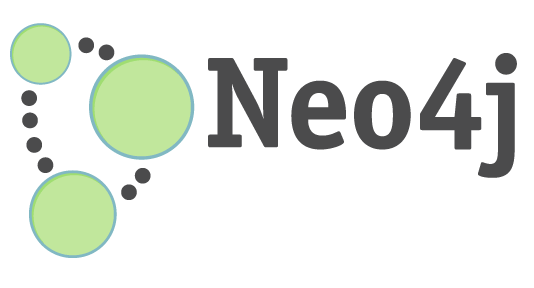
\includegraphics[scale=0.3]{img/part1/4.12}
    \caption{Logo Neo4J}
\end{figure}

\newpage 
\begin{center}
\color[rgb]{0.2, 0.6, 0.2} D'autres base de données peuvent proposées plusieurs services en même temps comme: 
\end{center} 

\paragraph{Amazon DynamoDB:}
DynamoDB utilise un modèle de base de données NoSQL, qui n'est pas relationnel, ce qui permet d'avoir des documents, des graphiques parmi ses modèles de données.  Chaque requête DynamoDB est exécutée par une clé primaire identifiée par l'utilisateur, qui identifie de manière unique chaque élément. Il libère également les clients du fardeau de l'exploitation et de la mise à l'échelle d'une base de données distribuée. Ainsi, le provisionnement matériel, l'installation, la configuration, la réplication, le patch logiciel, la mise à l'échelle des clusters, etc. sont gérés par Amazon.

Caractéristiques :
\begin{itemize}[label=\ding{51}]
\item Haute évolutivité.
\item Plage de hachage pour l'indexation d'une plage de valeurs.
\item Stockage des données dans les partitions.
\item Utilise JSON comme protocole de transport et non comme format de stockage.
\end{itemize}


